\documentclass{standalone}
\usepackage{tikz}
\usetikzlibrary{patterns, positioning}
\usetikzlibrary{shapes.misc}
\usepackage[outline]{contour}
\contourlength{1.5pt} 


\begin{document}
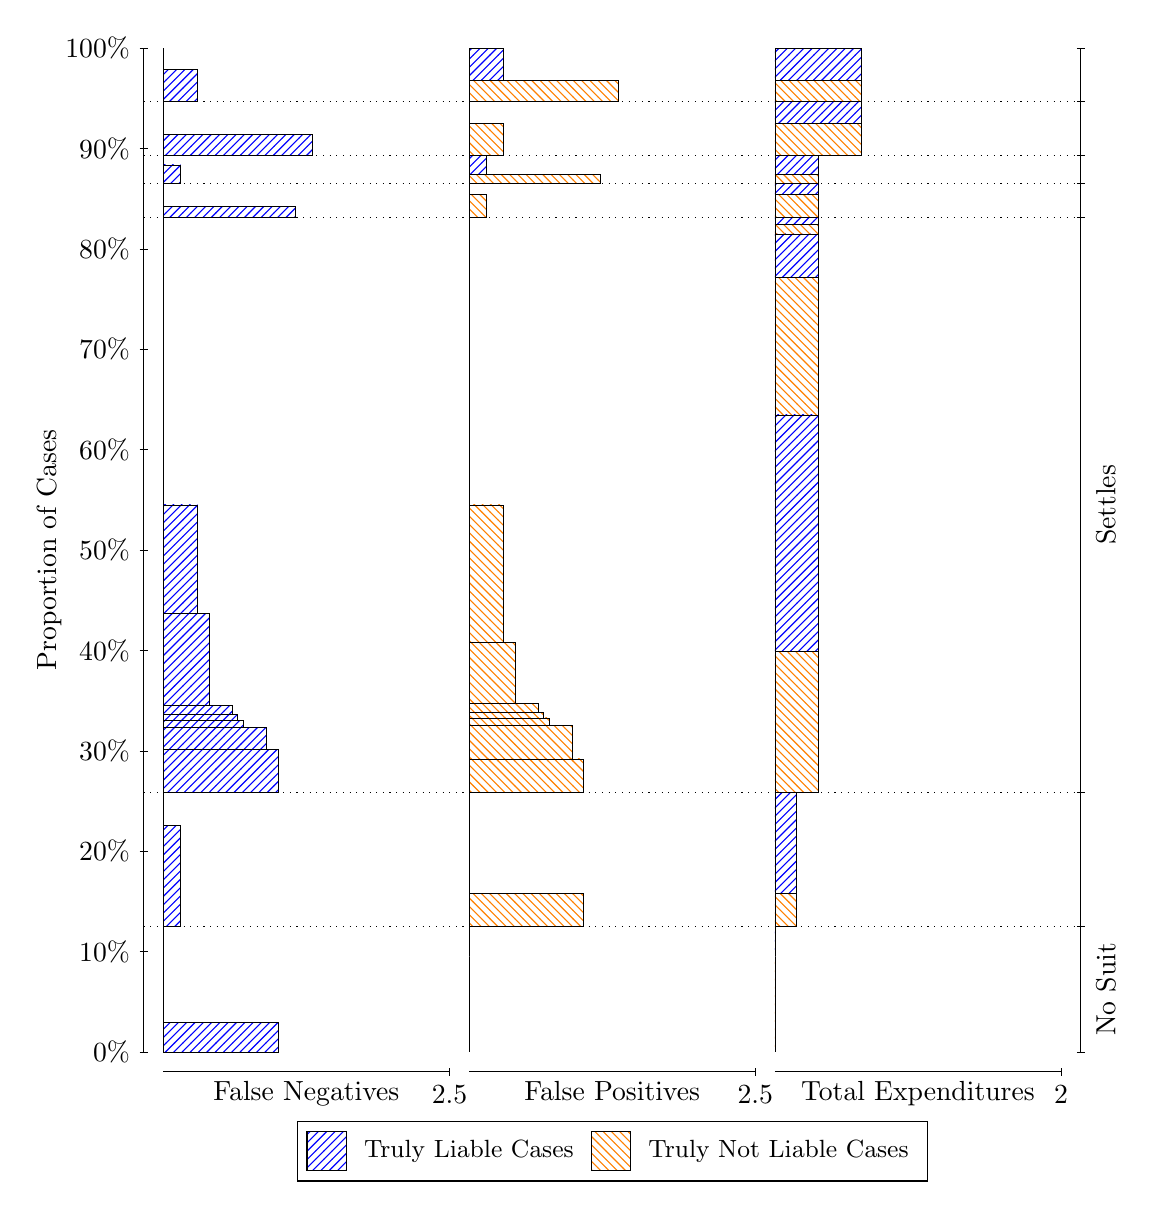
\begin{tikzpicture}
\draw[black, very thin] (1.5,1.75) -- (1.5,14.5);
\node[rotate=90, text=black, anchor=center] at (0.3, 8.125) {Proportion of Cases};
\draw[black, very thin] (1.45,1.75) -- (1.55,1.75);
\node[text=black, anchor=east] at (1.45, 1.75) {0\%};
\draw[black, very thin] (1.45,3.025) -- (1.55,3.025);
\node[text=black, anchor=east] at (1.45, 3.025) {10\%};
\draw[black, very thin] (1.45,4.3) -- (1.55,4.3);
\node[text=black, anchor=east] at (1.45, 4.3) {20\%};
\draw[black, very thin] (1.45,5.575) -- (1.55,5.575);
\node[text=black, anchor=east] at (1.45, 5.575) {30\%};
\draw[black, very thin] (1.45,6.85) -- (1.55,6.85);
\node[text=black, anchor=east] at (1.45, 6.85) {40\%};
\draw[black, very thin] (1.45,8.125) -- (1.55,8.125);
\node[text=black, anchor=east] at (1.45, 8.125) {50\%};
\draw[black, very thin] (1.45,9.4) -- (1.55,9.4);
\node[text=black, anchor=east] at (1.45, 9.4) {60\%};
\draw[black, very thin] (1.45,10.675) -- (1.55,10.675);
\node[text=black, anchor=east] at (1.45, 10.675) {70\%};
\draw[black, very thin] (1.45,11.95) -- (1.55,11.95);
\node[text=black, anchor=east] at (1.45, 11.95) {80\%};
\draw[black, very thin] (1.45,13.225) -- (1.55,13.225);
\node[text=black, anchor=east] at (1.45, 13.225) {90\%};
\draw[black, very thin] (1.45,14.5) -- (1.55,14.5);
\node[text=black, anchor=east] at (1.45, 14.5) {100\%};

\draw[black, very thin] (13.4,1.75) -- (13.4,14.5);
\draw[black, very thin] (13.35,1.75) -- (13.45,1.75);
\node[anchor=west] at (13.35, 1.75) {};
\draw[black, very thin] (13.35,3.3411) -- (13.45,3.3411);
\node[anchor=west] at (13.35, 3.3411) {};
\draw[black, very thin] (13.35,5.0462) -- (13.45,5.0462);
\node[anchor=west] at (13.35, 5.0462) {};
\draw[black, very thin] (13.35,12.35) -- (13.45,12.35);
\node[anchor=west] at (13.35, 12.35) {};
\draw[black, very thin] (13.35,12.778) -- (13.45,12.778);
\node[anchor=west] at (13.35, 12.778) {};
\draw[black, very thin] (13.35,13.134) -- (13.45,13.134);
\node[anchor=west] at (13.35, 13.134) {};
\draw[black, very thin] (13.35,13.819) -- (13.45,13.819);
\node[anchor=west] at (13.35, 13.819) {};
\draw[black, very thin] (13.35,14.5) -- (13.45,14.5);
\node[anchor=west] at (13.35, 14.5) {};

\draw[black, very thin, pattern color=blue, pattern=north east lines] (1.75,1.75) rectangle (3.2033,2.1282);
\draw[black, very thin, pattern color=orange, pattern=north west lines] (1.75,2.1282) rectangle (1.75,3.3411);
\draw[black, very thin, pattern color=blue, pattern=north east lines] (1.75,3.3411) rectangle (1.968,4.628);
\draw[black, very thin, pattern color=orange, pattern=north west lines] (1.75,4.628) rectangle (1.75,5.0462);
\draw[black, very thin, pattern color=blue, pattern=north east lines] (1.75,5.0462) rectangle (3.2033,5.5963);
\draw[black, very thin, pattern color=blue, pattern=north east lines] (1.75,5.5963) rectangle (3.058,5.8716);
\draw[black, very thin, pattern color=blue, pattern=north east lines] (1.75,5.8716) rectangle (2.7673,5.9652);
\draw[black, very thin, pattern color=blue, pattern=north east lines] (1.75,5.9652) rectangle (2.6947,6.034);
\draw[black, very thin, pattern color=blue, pattern=north east lines] (1.75,6.034) rectangle (2.622,6.1493);
\draw[black, very thin, pattern color=blue, pattern=north east lines] (1.75,6.1493) rectangle (2.3313,7.3217);
\draw[black, very thin, pattern color=blue, pattern=north east lines] (1.75,7.3217) rectangle (2.186,8.6987);
\draw[black, very thin, pattern color=orange, pattern=north west lines] (1.75,8.6987) rectangle (1.75,12.35);
\draw[black, very thin, pattern color=blue, pattern=north east lines] (1.75,12.35) rectangle (3.4213,12.487);
\draw[black, very thin, pattern color=orange, pattern=north west lines] (1.75,12.487) rectangle (1.75,12.778);
\draw[black, very thin, pattern color=blue, pattern=north east lines] (1.75,12.778) rectangle (1.968,13.016);
\draw[black, very thin, pattern color=orange, pattern=north west lines] (1.75,13.016) rectangle (1.75,13.134);
\draw[black, very thin, pattern color=blue, pattern=north east lines] (1.75,13.134) rectangle (3.6393,13.407);
\draw[black, very thin, pattern color=orange, pattern=north west lines] (1.75,13.407) rectangle (1.75,13.819);
\draw[black, very thin, pattern color=blue, pattern=north east lines] (1.75,13.819) rectangle (2.186,14.228);
\draw[black, very thin, pattern color=orange, pattern=north west lines] (1.75,14.228) rectangle (1.75,14.5);
\draw[black, very thin, pattern color=orange, pattern=north west lines] (5.6333,1.75) rectangle (5.6333,2.9629);
\draw[black, very thin, pattern color=blue, pattern=north east lines] (5.6333,2.9629) rectangle (5.6333,3.3411);
\draw[black, very thin, pattern color=orange, pattern=north west lines] (5.6333,3.3411) rectangle (7.0867,3.7592);
\draw[black, very thin, pattern color=blue, pattern=north east lines] (5.6333,3.7592) rectangle (5.6333,5.0462);
\draw[black, very thin, pattern color=orange, pattern=north west lines] (5.6333,5.0462) rectangle (7.0867,5.4724);
\draw[black, very thin, pattern color=orange, pattern=north west lines] (5.6333,5.4724) rectangle (6.9413,5.8991);
\draw[black, very thin, pattern color=orange, pattern=north west lines] (5.6333,5.8991) rectangle (6.6507,5.9927);
\draw[black, very thin, pattern color=orange, pattern=north west lines] (5.6333,5.9927) rectangle (6.578,6.0615);
\draw[black, very thin, pattern color=orange, pattern=north west lines] (5.6333,6.0615) rectangle (6.5053,6.1768);
\draw[black, very thin, pattern color=orange, pattern=north west lines] (5.6333,6.1768) rectangle (6.2147,6.9488);
\draw[black, very thin, pattern color=orange, pattern=north west lines] (5.6333,6.9488) rectangle (6.0693,8.6973);
\draw[black, very thin, pattern color=blue, pattern=north east lines] (5.6333,8.6973) rectangle (5.6333,12.35);
\draw[black, very thin, pattern color=orange, pattern=north west lines] (5.6333,12.35) rectangle (5.8513,12.641);
\draw[black, very thin, pattern color=blue, pattern=north east lines] (5.6333,12.641) rectangle (5.6333,12.778);
\draw[black, very thin, pattern color=orange, pattern=north west lines] (5.6333,12.778) rectangle (7.3047,12.896);
\draw[black, very thin, pattern color=blue, pattern=north east lines] (5.6333,12.896) rectangle (5.8513,13.134);
\draw[black, very thin, pattern color=orange, pattern=north west lines] (5.6333,13.134) rectangle (6.0693,13.547);
\draw[black, very thin, pattern color=blue, pattern=north east lines] (5.6333,13.547) rectangle (5.6333,13.819);
\draw[black, very thin, pattern color=orange, pattern=north west lines] (5.6333,13.819) rectangle (7.5227,14.091);
\draw[black, very thin, pattern color=blue, pattern=north east lines] (5.6333,14.091) rectangle (6.0693,14.5);
\draw[black, very thin, pattern color=orange, pattern=north west lines] (9.5167,1.75) rectangle (9.5167,2.9629);
\draw[black, very thin, pattern color=blue, pattern=north east lines] (9.5167,2.9629) rectangle (9.5167,3.3411);
\draw[black, very thin, pattern color=orange, pattern=north west lines] (9.5167,3.3411) rectangle (9.7892,3.7592);
\draw[black, very thin, pattern color=blue, pattern=north east lines] (9.5167,3.7592) rectangle (9.7892,5.0462);
\draw[black, very thin, pattern color=orange, pattern=north west lines] (9.5167,5.0462) rectangle (10.062,6.8334);
\draw[black, very thin, pattern color=blue, pattern=north east lines] (9.5167,6.8334) rectangle (10.062,9.8422);
\draw[black, very thin, pattern color=orange, pattern=north west lines] (9.5167,9.8422) rectangle (10.062,11.591);
\draw[black, very thin, pattern color=blue, pattern=north east lines] (9.5167,11.591) rectangle (10.062,12.141);
\draw[black, very thin, pattern color=orange, pattern=north west lines] (9.5167,12.141) rectangle (10.062,12.256);
\draw[black, very thin, pattern color=blue, pattern=north east lines] (9.5167,12.256) rectangle (10.062,12.35);
\draw[black, very thin, pattern color=orange, pattern=north west lines] (9.5167,12.35) rectangle (10.062,12.641);
\draw[black, very thin, pattern color=blue, pattern=north east lines] (9.5167,12.641) rectangle (10.062,12.778);
\draw[black, very thin, pattern color=orange, pattern=north west lines] (9.5167,12.778) rectangle (10.062,12.896);
\draw[black, very thin, pattern color=blue, pattern=north east lines] (9.5167,12.896) rectangle (10.062,13.134);
\draw[black, very thin, pattern color=orange, pattern=north west lines] (9.5167,13.134) rectangle (10.607,13.547);
\draw[black, very thin, pattern color=blue, pattern=north east lines] (9.5167,13.547) rectangle (10.607,13.819);
\draw[black, very thin, pattern color=orange, pattern=north west lines] (9.5167,13.819) rectangle (10.607,14.091);
\draw[black, very thin, pattern color=blue, pattern=north east lines] (9.5167,14.091) rectangle (10.607,14.5);
\draw[black, dotted] (1.5,3.3411) -- (13.4,3.3411);
\draw[black, dotted] (1.5,5.0462) -- (13.4,5.0462);
\draw[black, dotted] (1.5,12.35) -- (13.4,12.35);
\draw[black, dotted] (1.5,12.778) -- (13.4,12.778);
\draw[black, dotted] (1.5,13.134) -- (13.4,13.134);
\draw[black, dotted] (1.5,13.819) -- (13.4,13.819);
\draw[black, very thin] (1.75,1.5) -- (5.3833,1.5);
\node[text=black, anchor=north] at (3.5667, 1.5) {False Negatives};
\draw[black, very thin] (5.3833,1.45) -- (5.3833,1.55);
\node[text=black, anchor=north] at (5.3833, 1.45) {2.5};

\draw[black, very thin] (5.6333,1.5) -- (9.2667,1.5);
\node[text=black, anchor=north] at (7.45, 1.5) {False Positives};
\draw[black, very thin] (9.2667,1.45) -- (9.2667,1.55);
\node[text=black, anchor=north] at (9.2667, 1.45) {2.5};

\draw[black, very thin] (9.5167,1.5) -- (13.15,1.5);
\node[text=black, anchor=north] at (11.333, 1.5) {Total Expenditures};
\draw[black, very thin] (13.15,1.45) -- (13.15,1.55);
\node[text=black, anchor=north] at (13.15, 1.45) {2};

\node[text=black, centered, rotate=90] at (13.72, 2.5455) {\contour{white}{No Suit}};

\node[text=black, centered, rotate=90] at (13.72, 8.698) {\contour{white}{Settles}};





\draw (7.449999999999999,1.5) node[draw=none] (baseCoordinate) {};
\begin{scope}[align=center]
        \matrix[scale=0.5, draw=black, below=0.5cm of baseCoordinate, nodes={draw}, column sep=0.1cm]{
            \node[rectangle, draw, minimum width=0.5cm, minimum height=0.5cm, pattern color=blue, pattern=north east lines] {}; &
            \node[draw=none, font=\small, text=black] (B) {Truly Liable Cases}; &
            \node[rectangle, draw, minimum width=0.5cm, minimum height=0.5cm, pattern color=orange, pattern=north west lines] {}; &
            \node[draw=none, font=\small, text=black] (B) {Truly Not Liable Cases}; \\
            };
\end{scope}

\end{tikzpicture}
\end{document}